\section*{Appendix 1: Radiation Cloud Modelling}\label{sec:radiation}
\noindent The radiation cloud diffusion process is modelled using the Smoluchowski drift-diffusion equation, 
\begin{eqnarray}
\frac{D \text{Rad}({\bf z}, \tau)}{D \tau}=\kappa \triangledown^2 \text{Rad}({\bf z},\tau)-\text{Rad}({\bf z},\tau)\triangledown \cdot {\bf w}({\bf z},\tau)+\sigma({\bf z},\tau)
\label{clouddyns}
\end{eqnarray}
where $D$ is the material derivative, $\text{Rad}({\bf z},\tau)$ is the radiation cloud intensity at location ${\bf z}=(x,y)$ at time $\tau$, $\kappa$ is a fixed diffusion coefficient and $\sigma$ is the radiation source(s) emission rate. The diffusion equation is solved on a regular grid defined across the environment with grid coordinates $G$ (as defined in Section \ref{sec:model}).  Furthermore, the grid is solved at discrete time instances $\tau$.  The cloud is driven by stochastic wind forces which vary both spatially and temporally.  These forces induce anisotropy into the cloud diffusion process  proportional to the local average wind velocity, ${\bf w}({\bf z},\tau)$.  The wind velocity is drawn from two independent Gaussian processes (GP), one GP for each Cartesian coordinate axis, $w_i({\bf z},\tau)$, of ${\bf w}({\bf z},\tau)$.  The GP captures both the spatial distribution of the wind velocity and the dynamic process resulting from shifting wind patterns (e.g., short term gusts and longer term variations). 

%\todo{STEVE: can you please add back the TEX text to the paragraphs to make it a more %complete description and check if picture below fits the flow}
In our simulation, each spatial wind velocity component is modelled by an isotropic squared-exponential GP covariance function \cite{rasmussen06}, $K$, with fixed input and output scales, $l$ and $\mu$, respectively (although any covariance function can be substituted),
\begin{eqnarray*}
K({\bf z},{\bf z}^\prime)=\mu^2\exp -({\bf z}-{\bf z}^\prime)^T {\bf P}^{-1}({\bf z}-{\bf z}^\prime)
\end{eqnarray*}
where ${\bf P}$ is a diagonal covariance matrix with diagonal elements $l^2$.  This choice of covariance function generates wind conditions which vary smoothly in both magnitude and direction across the terrain.  Furthermore, as wind conditions may change over time we introduce a temporal correlation coefficient, $\rho$, to the covariance function.  Thus, for a single component, $w_i$, of ${\bf w}$, defined over grid $G$ at times $\tau$ and $\tau^\prime$, the wind process covariance function is, $\text{Cov}(w_i({\bf z},\tau),w_i({\bf z^\prime},\tau^\prime))=\rho(\tau,\tau^\prime) K({\bf z},{\bf z}^\prime)$.  We note that, when $\rho=1$ the wind velocities are time invariant (although spatially variant).  Values of $\rho<1$ model wind conditions that change over time.

Using the above model, we are able to create a moving radiation cloud. This poses a real challenge both for the HQ ($PA$ and $H$) and the responders on the ground, as the predictions they make of where the cloud will move to will be prone to uncertainty both due to the simulated wind speed and direction.  While it is possible to use radiation readings provided by first responders on the ground, as they move in the disaster space, in our trials, we assumed that these readings are coming from sensors already embedded in the environment to allow the team to focus on path planning for task allocation (which is the focus of this paper) rather than for radiation monitoring. Hence, using such sensor readings, the prediction algorithm provided in Appendix \ref{sec:appendix} is then used to provide estimates of the radiation levels across  the disaster space during the game. These estimates are displayed as a heat map as described in the previous section.

\section*{Appendix 1: Predictive Model of Radiation Cloud}\label{sec:appendix}

Predictions of the clouds location are performed using a latent force model (LFM) \cite{reece10,reece14}.  The LFM is a Markov model that allows the future state of the cloud and wind conditions to be predicted efficiently from the current state.  Predictions are computed using the Extended Kalman filter (EKF) which has a linear computational complexity with regard to the time interval the dynamics are predicted forward.~\footnote{The EKF accommodates the nonlinearities in the radiation dynamics expressed through equation (\ref{clouddyns}).}  The EKF estimates provide both the mean and variance of the state of the cloud and wind conditions.  Figure~\ref{radiation_screen_shots} shows example cloud simulations for slow varying (i.e. $\rho=0.99$) and gusty (i.e. $\rho=0.90$) wind conditions.  The left panes in each subfigure show the ground truth simulation obtained by sampling from the LFM.  The middle panes show the mean of the cloud and wind conditions and the right panes show the uncertainty in the conditions.

The radiation cloud can be monitored using a number of sensors on the ground that collect readings of the radiation cloud intensity and, optionally, wind velocity every minute of the game. These {\it monitor agents} can be at fixed locations or they can be mobile agents equipped with geiger-counters that inform the user and commander of the local radiation intensity.  The mobile agents can be directed to take measurements with greatest information gain in the radiation cloud intensity.  The measurements can be folded into the EKF and this refines estimates of both the radiation cloud and wind conditions across the grid.  Figure~\ref{radiation_screen_shots} shows the impact of such measurements on the uncertainty of the cloud and wind conditions.  The current location of the monitors are shown as black dots in the upper row of panes in both subfigures.  The right most panes show the relative uncertainty in both the cloud and wind conditions as a result of current and past measurements.  Figure~\ref{radiation_screen_shots}(a) shows slow varying wind conditions in which case the radiation cloud can be interpolated accurately using sparse sensor measurements and the LFM model.  Alternatively, during gusty conditions the radiation cloud model is more uncertain far from the locations where recent measurements have been taken, as shown in Figure~\ref{radiation_screen_shots}(b).
\begin{figure}[ht] \begin{center}
    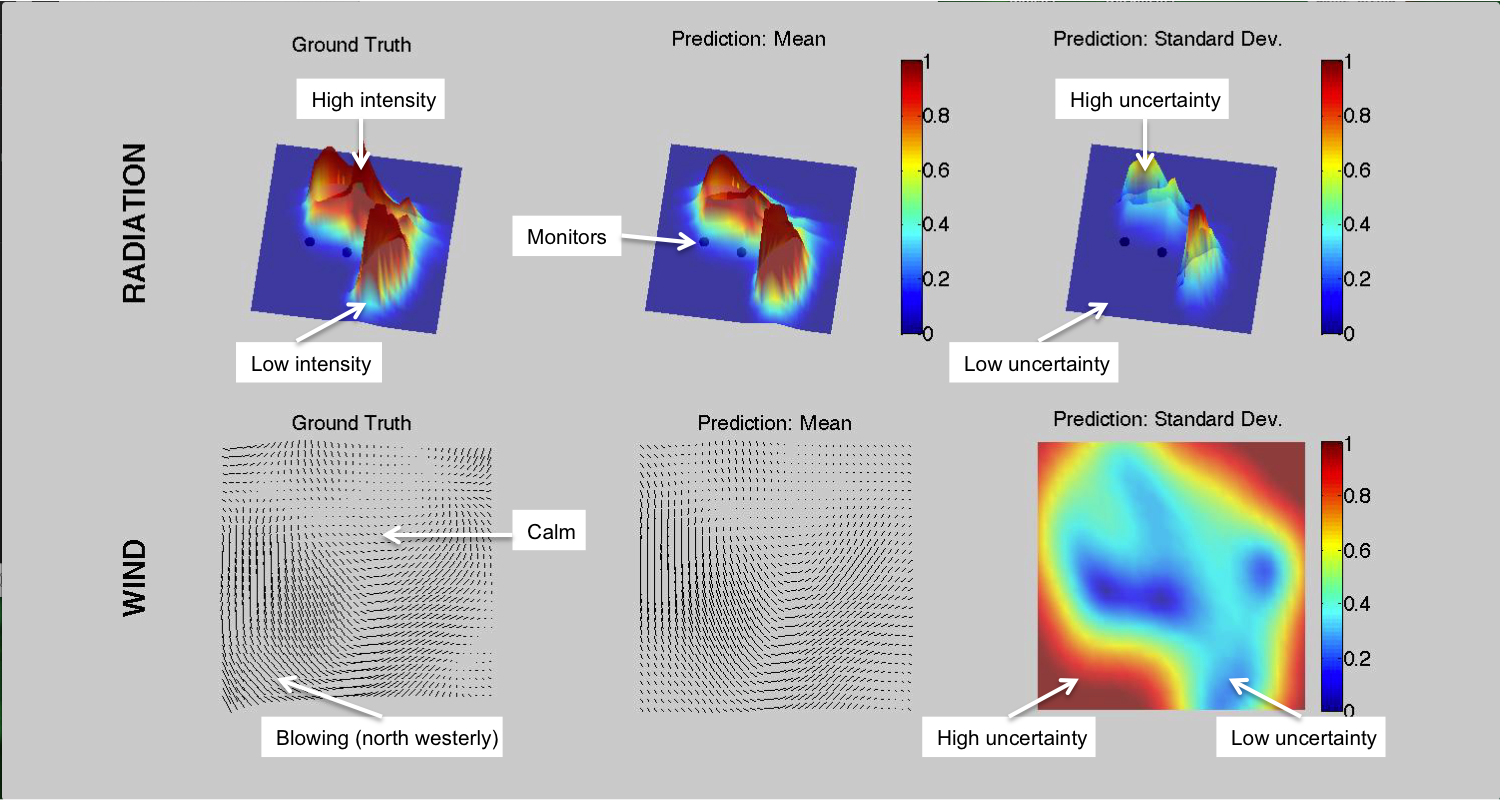
\includegraphics[width=0.90\textwidth]{figures/radiation_ss_calm_annotated.png}\\
    (a) Slowly varying wind conditions\\ \ \\
    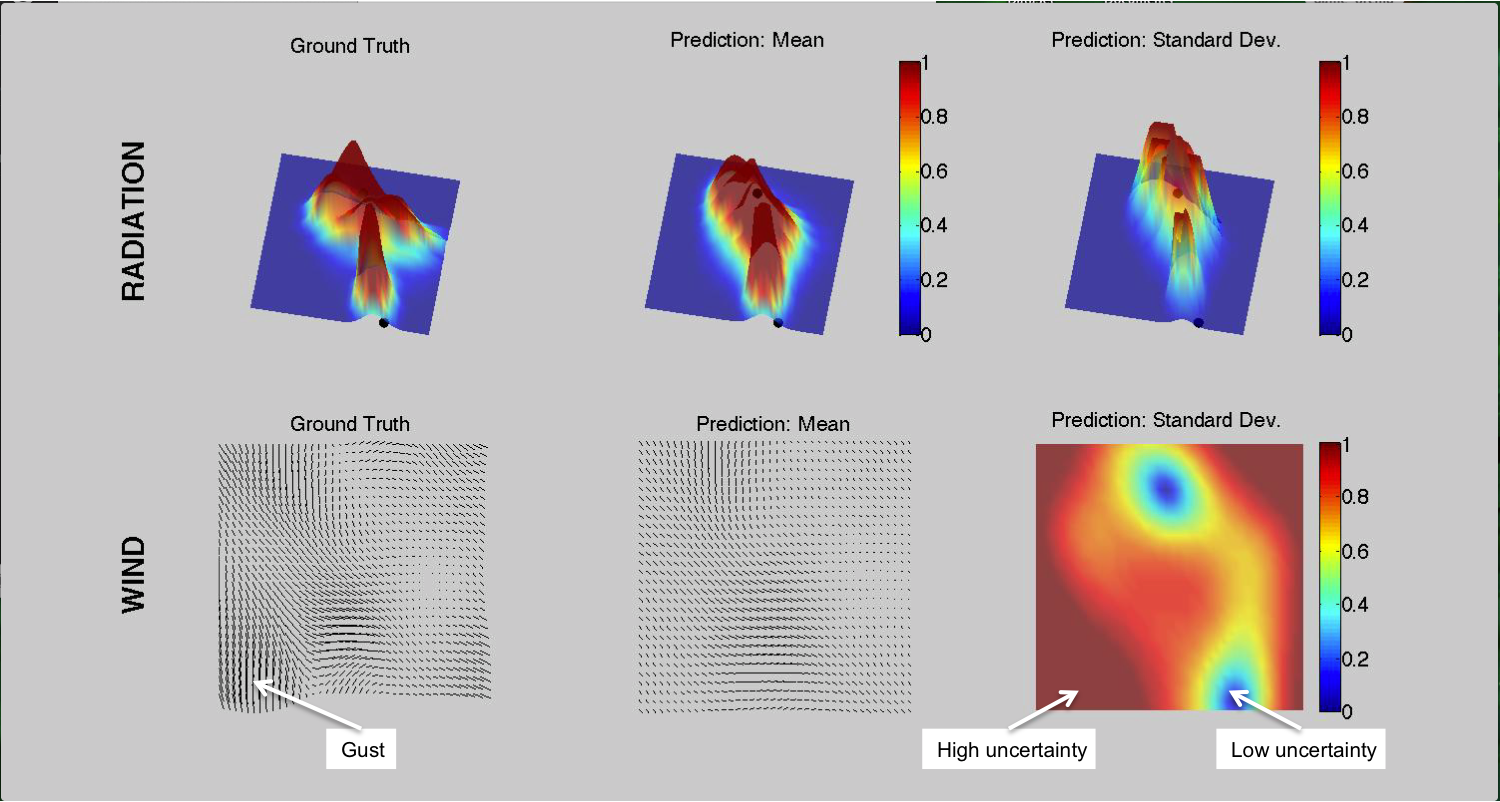
\includegraphics[width=0.90\textwidth]{figures/radiation_ss_gust_annotated.png}\\
    (b) Gusty wind conditions 
\caption{\label{radiation_screen_shots} Radiation and wind simulation ground truth and EKF estimates obtained using measurements from monitor agents (black dots).  Left most panes are ground truth radiation and wind conditions, the middle panes are corresponding estimates and right most panes are state uncertainties:  (a) invariant and (b) gusty wind conditions.}
\end{center}
\end{figure}
